\documentclass[]{article}
% Grundlegende Dokumenteinstellungen
\usepackage[a4paper,left=3cm,right=3cm,top=2cm,bottom=4cm,bindingoffset=5mm]{geometry}
% Datum in deutscher Formatierung
\usepackage[german]{babel}
% UTF-8 als Zeichencodierung verwenden
\usepackage[utf8]{inputenc}
\usepackage{booktabs}
% Farben definieren
\usepackage[svgnames]{xcolor}
\definecolor{LinkColor}{RGB}{0,128,128}
% Hyperlinks
\usepackage[colorlinks=true, allcolors=LinkColor, pdfborder={0 0 0}]{hyperref}

% Applesymbole, z.B. auf der Commandtaste
\usepackage{applekeys}
% Codeblöcke
\usepackage{minted}
% Rahmen um Codeblöcke zeichnen. Benutzen mit \begin{bashcode}...
\newminted{bash}{frame=single,framesep=10pt,fontsize=\small}

% (externe) Grafiken 
\usepackage{graphicx}
\usepackage{filecontents}
% Bibliothek mit Verweisen bei Zitaten
\usepackage[backend=biber]{biblatex}
\addbibresource{FullstackentwicklungMitMacOS.bib}

% Unterstützung für Sonderzeichen, wie z.B. > < usw.
\usepackage[T1]{fontenc}

% Unterstützung für Inline-Codeblöcke
\newcommand{\code}[1]{\texttt{#1}}

% Abstand und Einzug bei Absätzen
\setlength{\parindent}{0pt}
\setlength{\parskip}{1em}


%opening
\title{Fullstackentwicklung mit MacOS}
\author{Bastian Nolte}


\begin{document}

\maketitle
\section{Einleitung}
Dieser Artikel beschreibt die Installation und Konfiguration von verbreiteten Werkzeugen zur Fullstackentwicklung unter MacOS, am Beispiel von Java und JavaScript/TypeScript.

Das Dokument gliedert sich in zwei Teile. Der erste Teil beschreibt allgemein die Installation und Konfiguration der Entwicklungstoolchain. Der zweite Teil geht dann auf die Besonderheiten bei der CSS-Versicherung ein.

\section{Vorbedingungen}
Es wird ein Computer mit MacOS als Betriebssystem, sowie ein grundlegendes Verständnis dieses Betriebssystems vorausgesetzt.

\section{Xcode}
\href{https://developer.apple.com/xcode/}{Xcode} ist eine integrierte Entwicklungsumgebung für macOS mit einer Reihe von Softwareentwicklungswerkzeugen, die von Apple für die Entwicklung von Software für macOS, iOS, watchOS und tvOS entwickelt wurden.

Installiere Xcode über den AppStore von Apple.
\subsection{Xcode command line tools}
Xcode verfügt auch über einen Satz von Kommandozeilenwerkzeugen. Diese installierst Du am besten über das Terminal. Das Terminal kannst Du öffnen, indem Du \cmdkey+Leertaste drückst und dann \code{terminal} eingibst und \returnkey\, drückst.

Danach kann die Installation der \code{Xcode  command line tools} wie folgt durchgeführt werden.
\begin{bashcode}
xcode-select --install
\end{bashcode}

\section{Paketmanager}
MacOS bringt keinen eigenen Paketmanager mit, wie man ihn von anderen Unix-Derivaten kennt. Daher haben es sich verschiedene Projekte zur Aufgabe gemacht, diese Lücke zu füllen.

Die folgende Liste liefert einen Überblick aktueller Paketmanager im März 2019.

\begin{tabular}[t]{lll}
	\toprule
	Mac Paketmanager & Pakete & Benötigt Rootrechte \\
	\midrule
	Homebrew & 4635 & Nein \\
	Homebrew Cask & 4051 & Nein \\
	Nix package manager & 15858 & Nein \\
	pkgsrc & 18560 & Ja \\
	MacPorts & 20572 & Ja \\
	\bottomrule
\end{tabular}

Die Informationen wurden von der Seite \href{https://www.slant.co/topics/511/~best-mac-package-managers#3}{Slant...  What are the best Mac package managers?} bezogen.

\subsection{Homebrew installieren}
Homebrew kann einfach über das Terminal installiert werden.

Die Installation erfolgt durch Eingabe des folgenden Kommandos im soeben geöffneten Terminal:
\begin{bashcode}
HOMEBREW_URL='https://raw.githubusercontent.com/Homebrew/install/master/install'
/usr/bin/ruby -e "$(curl -fsSL $HOMEBREW_URL)"
\end{bashcode}

\subsection{Die wichtigsten Homebrewkommandos}
\begin{bashcode}
# Nach einem bestimmten Paket suchen
brew search <paketname> 

# Das OpenSource-Paket mit dem Namen <paketname> installieren
brew install <paketname>

# Ein nicht OpenSource-Paket installieren,  z.B. kommerzielle MacOS-Apps.
brew cask install <paketname>  

# Alle bereits installierten Pakete und deren mitinstallierte Abhängigkeiten 
# in einer Baumansicht auflisten.
brew deps --tree --installed

# Alle installierten Pakete in einer flachen Ansicht auflisten
brew list && brew cask list

# Informationen zu einem bereits installierten Paket erhalten
brew info <paketname> 
\end{bashcode}

Weitere Informationen findest Du auf der \href{https://brew.sh/index_de}{Homepage} des Homebrew-Projektes.

\section{iTerm2}
\href{https://www.iterm2.com/}{iTerm2} ist ein Open-Source-Ersatz für Apples Terminal. Es ist sehr anpassungsfähig und verfügt über viele nützliche Funktionen.

Du kannst es wie folgt installieren:
\begin{bashcode}
brew cask install iterm2
\end{bashcode}

Du startest iTerm2 indem Du \cmdkey+Leertaste drückst und dann \code{iterm} eingibst und \returnkey\, drückst. Eine Darstellung der Vorteile, dies sich durch den Einsatz von \code{iTerm} ergeben findest Du auf der \href{https://www.iterm2.com/features.html}{Featureseite} von iTerm.

\subsection{Tastenkombinationen anpassen}
Wahrscheinlich kennst Du die Tastenkombinationen mit denen Du wortweise (\optkey) vor- und zurückspringen, beziehungsweise zum Anfang und Ende der Zeile (\cmdkey) navigieren kannst.

Auch iTerm kannst Du so einstellen. Öffne dazu die iTerm2-Einstellungen (\cmdkey +,) und navigiere dann zu \code{Profile} > \code{Schlüssel} und klicke  auf das Symbol +  um eine neue Tastenkombination hinzufügen.

\begin{tabular}[t]{lll}
	\toprule
	Keyboard Shortcut & Action & Send \\
	\midrule
	\cmdkey \textleftarrow & Send escape sequence & OH \\
	\cmdkey \textrightarrow & Send escape sequence & OF \\
	\optkey \textleftarrow & Send escape sequence & b \\
	\optkey \textrightarrow & Send escape sequence & f \\
\end{tabular}

Nun kannst Du wortweise vor- und zurück, sowie an den Anfang und das Ende der Zeile navigieren.

\section{Z-Shell}
Die Z-Shell, die Du vielleicht unter dem Namen zsh kennst, ist eine Unix-Shell, die auf der Standard-Shell für macOS aufbaut und diese um weitere nützliche Funktionen erweitert. 

Installieren kannst Du die zsh durch Eingabe folgenden Befehls:
\begin{bashcode}
brew install zsh
\end{bashcode}

Du solltest ein Framework mit der zsh installieren, da es die Konfiguration und den Einsatz von Plugins und Themes deutlich erleichtert. Es gibt zwei besonders populäre Frameworks, \href{https://github.com/robbyrussell/oh-my-zsh}{Oh My Zsh} und \href{https://github.com/sorin-ionescu/prezto}{Prezto}.
Bitte beachte, dass Du nur ein Framework und nicht beide installieren solltest, da Du sonst mit Problemen rechnen musst.

\subsection{Oh My Zsh}
Ich habe mich dafür entschieden \code{Oh My Zsh} einzusetzen. Um es zu installieren, gibst Du folgenden Befehl in Dein Terminal ein.
\begin{bashcode}
sh -c "$(curl -fsSL https://raw.githubusercontent.com/robbyrussell\
/oh-my-zsh/master/tools/install.sh)"
chsh -s $(which zsh) # Setzt die zsh als Standardshell.
\end{bashcode}

Ein Upgrade kannst Du mit dem Kommando \code{upgrade\_oh\_my\_zsh} durchführen. Starte \code{iTerm2} neu, um zsh zu aktivieren.

\subsection{Oh My Zsh anpassen}
Die Einstellungen von \code{Oh My Zsh} nach der Installation sind schon recht brauchbar. Es bietet Dir allerdings diverse Möglichkeiten sein Aussehen und Verhalten an Deine Anforderungen anzupassen. Wie das funktioniert kannst Du im \href{https://github.com/robbyrussell/oh-my-zsh/wiki}{Wiki} nachlesen.

Wir wollen für den Anfang einige Plugins installieren. Öffne hierzu die Datei \code{\~\//.zshrc}, finde die Zeile die mit \code{plugins=} beginnt und trage Plugins wie folgt ein:
\begin{bashcode}
plugins=(
  colored-man 
  colorize  
  docker 
  git 
  github 
  history 
  mvn 
  ng 
  node 
  npm 
  osx 
  zsh-syntax-highlighting
)
\end{bashcode}
Ob Du alle Plugins in eine Zeile schreibst oder jedes in eine eigene Zeile, ist hierbei unerheblich. Wichtig ist nur, dass Du die Plugins durch mindestens ein Leerzeichnen voneinander trennst.

Zudem könnte es sich als praktisch erweisen, in der Eingabehistorie weiter zurückblicken zu können. Dies kannst Du erreichen, indem Du Deiner Konfigurationsdatei folgende Zeilen hinzufügst.

\begin{bashcode}
export HISTSIZE=10000
export HISTFILESIZE=10000
\end{bashcode}

Die Änderungen werden wirksam, sobald Du iTerm neu gestartet hast.


\section{Secure Shell}
Secure Shell oder SSH bezeichnet sowohl ein Netzwerkprotokoll als auch entsprechende Programme, mit deren Hilfe man auf eine sichere Art und Weise eine verschlüsselte Netzwerkverbindung mit einem entfernten Gerät herstellen kann. Häufig wird diese Methode verwendet, um lokal eine entfernte Kommandozeile verfügbar zu machen, das heißt, auf einer lokalen Konsole werden die Ausgaben der entfernten Konsole ausgegeben und die lokalen Tastatureingaben werden an den entfernten Rechner gesendet. Genutzt werden kann dies beispielsweise zur Fernwartung eines in einem entfernten Rechenzentrum stehenden Servers.\cite{wikipediaSecureShell}
\subsection{Einen SSH-Schlüssel erzeugen}
Ein SSH-Schlüssel besteht aus einem Paar von Dateien. Eine davon beinhaltet den privaten Schlüssel, der niemals an Dritte weitergegeben werden sollte. Die andere beinhaltet den öffentlichen Schlüssel. Diesen öffentlichen Schlüssel kannst Du dazu verwenden Dich an Systemen anzumelden ohne Benutzername und Passwort eingeben zu müssen.

Ein Schlüsselpaar kann wie folgt erzeugt werden:
\begin{bashcode}
ssh-keygen -t rsa
\end{bashcode}

\subsection{Den öffentlichen Schlüssel in die Zwischenablage kopieren}
\begin{bashcode}
pbcopy < ~/.ssh/id_rsa.pub
\end{bashcode}

\subsection{Den öffenlichen Schlüssel übertragen}
Überträgt man den öffentlichen SSH-Schlüssel auf einen anderen Computer, z.B. einen Server und hinterlegt diesen dort, dann kann man sich künftig an diesen Server anmelden, ohne Benutzernamen und Passwort eingeben zu müssen.

Der Schlüssel kann mit folgendem Befehl übertragen und hinterlegt werden:
\begin{bashcode}
# ssh-copy-id -i ~/.ssh/key_rsa.pub <benutzername>@<servername oder ip>, z.B.
ssh-copy-id -i ~/.ssh/key_rsa.pub musterfrau@webserver.example.com
\end{bashcode}

\subsection{SSH-Schlüssel, Phassphrasen und der MacOS-Schlüsselbund}
Ich empfehle Dir Deine SSH-Schlüssel mit einer Passphrase zu versehen. Wenn Du darauf verzichtest, kann sich jede Person, die in den Besitz Deines privaten Schlüssels gelangt, mit Deinem Benutzeraccount anmelden und das an allen Systemen auf denen Du Deinen Schlüssel hinterlegt hast.

Normalerweise müsstest Du dann aber bei jeder Verwendung des Schlüssels Deine Passphrase eingeben. Dies kann schnell anstrengend werden oder - zum Beispiel bei der automatisierten Kommunikation zwischen zwei Computern - sogar unmöglich sein.

Dies kannst Du vermeiden, indem Du Deine privaten Schlüsselidentitäten dem SSH-Authentifizierungsagenten hinzufügst und die Passphrasen im Schlüsselbund Deines MacOS-Benutzers hinterlegst. 

\begin{bashcode}
# ssd-add fügt Deine SSH-Schlüsselidentitäten
# dem SSH authentication agent hinzu
# -K sorgt dafür, dass Deine Passphrases in Deinem Schlüsselbund hinterlegt werden.
ssh-add -K
\end{bashcode}

SSH-Schlüssel kannst Du auch nachträglich mit eine Passphrase versehen.
\begin{bashcode}
ssh-keygen -p
\end{bashcode}

\section{Git}
\href{https://git-scm.com/}{Git} ist eine freie Software zur verteilten Versionsverwaltung von Dateien.

Installiere Git durch Eingabe des folgenden Kommandozeilenbefehls.
\begin{bashcode}
brew install git
\end{bashcode}

Weitere Informationen zu Git, findest Du im umfassenden und kostenlosen Buch \href{https://git-scm.com/book/en/v2}{Pro Git} auf der Projekt Homepage, das auch in \href{https://git-scm.com/book/de/v2/}{deutscher Sprache} angeboten wird.

\subsection{Eine globale .gitignore-Datei anlegen}
Erzeuge eine \code{.gitignore}-Datei in Deinem Nutzerverzeichnis \code{\~} die Du global nutzen wirst. Diese könnte zum Beispiel, wie folgt aussehen:
\begin{bashcode}
 # See http://help.github.com/ignore-files/ for more about ignoring files.
 
# MacOS: Konfigurationsdateien für die Verzeichnisansicht
.DS_Store
Desktop.ini

# MacOS: Cache-Dateien für Miniaturansichten
._*
Thumbs.db

# Dateien, die auf externen Festplatten erscheinen können
.Spotlight-V100
.Trashes

# IntelliJ-IDEA
.idea/
/**/*.iml

# Eclipse-IDE
/**/.classpath
/**/.project
/**/.settings/
*.launch

 # Visual Studio Code IDE
.vscode/*
!.vscode/settings.json
!.vscode/tasks.json
!.vscode/launch.json
!.vscode/extensions.json

# node_modules - Über den Node Package Manager oder yarn verwaltete Abhängigkeiten
/node_modules

# Cache-Dateien des SASS-Compiler
.sass-cache/

# Maven-Kompilate
target/

# Code coverage Informationen
coverage/

\end{bashcode}

Registriere die Datei in Deiner globalen Git-Konfiguration, um die Einstellungen wirksam werden zu lassen.
\begin{bashcode}
git config --global core.excludesfile ~/.gitignore
\end{bashcode}

\section{Maven}
\href{https://maven.apache.org/}{Apache Maven} ist ein in Java geschriebenes Build-Management-Werkzeug. Maven versucht das Pattern "Konvention vor Konfiguration" konsequent für den gesamten Lebenszyklus einer Software abzubilden. Neben der Verwaltung von Abhängigkeiten, wird sowohl das Kompilieren und packen der Software, als auch die Verteilung unterstützt.

\subsection{Alternativen}
Neben Maven existieren noch diverse weitere Build-Management-Werkzeuge. Einen guten Überblick gibt der Artikel \href{https://jaxenter.de/8-build-tools-im-vergleich-ant-buildr-maven-bazel-buck-gradle-pants-sbt-41627}{Build-Tools im Vergleich} der Zeitschrift jaxenter.

Ich persönlich denke, dass (Stand 2019) \href{https://gradle.org/}{Gradle} besonders gut für die Arbeit in Java-Projekten geeignet ist. Gradle versucht die guten Seiten von Ant und Maven zu vereinen und ist dabei so erfolgreich, dass Google es als primäres Build-Tool bei der Entwicklung von Android verwendet. Statt XML nutzt Gradle eine domänenspezifische Sprache (DSL), die auf Groovy basiert. Skripte neigen deshalb dazu, wesentlich kürzer und klarer formuliert zu sein, als jene für Ant oder Maven.

Hinweis: Meines Wissens nach nutzt die CSS Versicherung zurzeit ausschliesslich Maven als Build-Management-Werkzeug für Java.

\subsection{Maven installieren}
Maven kann mit Homebrew wie folgt installiert werden.
\begin{bashcode}
brew install maven
\end{bashcode}



\section{npm}
\href{https://www.npmjs.com/}{npm} ist eines der führenden Build-Management-Werkzeuge in der JavaScript-Welt. Ähnlich wie Maven in der Javawelt, ist es hier sehr verbreitet. 

Aufgrund verschiedener Probleme, unter anderem mit der Verwaltung von indirekten Abhängigkeiten und wegen teils schlechter Performance, erlangte ein neues Build-Management-Werkzeug namens \href{https://yarnpkg.com}{Yarn} das Interesse der Entwicklergemeinde. Viele Gründe die für den Wechsel auf Yarn sprachen, sind in der aktuellen Version von npm nun aus der Welt geschaffen. Es findet eine Rege Diskussion in der Entwicklergemeinde darüber statt, welches der beiden Tool nun das bessere sei.

Hinweis: Meines Wissens nach nutzt die CSS Versicherung zurzeit ausschliesslich npm als Build-Management-Werkzeug für JavaSript und TypeScript.

\subsection{npm installieren}
npm kann mit Homebrew wie folgt installiert werden.
\begin{bashcode}
brew install npm
\end{bashcode}

\section{Entwicklungsumgebung}

    
- intellij-idea (ultimate)
- oracle-jdk

- google-chrome
- node
- angular-cli
- postman

\section{vim}
The Ultimate vimrc
git clone https://github.com/amix/vimrc.git \~{}/.vim\_runtime
sh \~{}/.vim\_runtime/install\_awesome\_vimrc.sh

\section{Kommandozeilenbefehle}
Liste nützlicher Kommandozeilenbefehle:
Schaue die Dokumentation zu einem Kommandozeilenbefehl an
\begin{bashcode}
man <kommandozeilenbefehl>
\end{bashcode}

Aktuellen Nutzer ausgeben
\begin{bashcode}
whoami
\end{bashcode}

Aktuellen Pfad (Verzeichnis) ausgeben
\begin{bashcode}
pwd
\end{bashcode}

Wechsle in ein Verzeichnis
\begin{bashcode}
#cd <verzeichnisname>, z.B.
cd /tmp
# Wechsle in das Nutzerverzeichnis (Heimatverzeichnis)
cd \~
# Wechsle zurück in das vorherige Verzeichnis
cd -
\end{bashcode}

Tip: Nutze <tab> und <tab><tab> für automatische Ergänzungen.

Verzeichnis erstellen
\begin{bashcode}
mkdir <verzeichnisname>
\end{bashcode}

Datei oder Verzeichnis verschieben
\begin{bashcode}
mv <quelle> <ziel>
\end{bashcode}

Datei oder Verzeichnis kopieren
\begin{bashcode}
cp <quelle> <ziel>
\end{bashcode}

Zeige den Inhalt einer Datei an:
\begin{bashcode}
# cat <dateiname>, z.B.
cat /var/log/meinserver.log
\end{bashcode}

Gebe die neuesten Inhalte einer Datei auf der Konsole aus
\begin{bashcode}
tail -f /var/log/messages
# Mit Unterstützung von Logrotate
tail -F /var/log/messages
\end{bashcode}

Alle Vorkommnisse eines regulären Ausdruckes in einer Datei ersetzen (substituieren), wobei die ursprüngliche Zustand in einer Kopie erhalten bleibt.
\begin{bashcode}
# sed -i.bu 's/<vorher>/<nachher>/g' <dateiname>, z.B.
sed -i.bu 's/Text/Hund/g' ./test.txt
\end{bashcode}

Finde alle Dateien mit bestimmten Merkmalen. Beispiel
\begin{bashcode}
# Dateien die in den letzten 10 Minuten geändert wurden 
find . -mmin -10
\end{bashcode}

Die Befehlshistorie anzeigen
\begin{bashcode}
history
\end{bashcode}

Den letzen Befehl nochmals als root ausführen
\begin{bashcode}
sudo !!
\end{bashcode}

Screen

Screensession aufzeichnen

\section{CSS-spezifische Einstellungen}
\subsection{Das DEVNET}
\subsection{GIT-Repositories verwenden}
Nicht alle GIT-Repositories stehen im DEVNET zur Verfügung. Informationen ... finden sich im ....

Zu dem gespiegelten Projekten findet sich jeweils ein Spiegelserver-Projekt auf dem Bitbucketserver. 
Für EBusiness wäre das entsprechend \href{https://git.css.ch/projects/EBUSINESS-MIRROR}{EBUSINESS-MIRROR}.

Klickt man auch der Bitbucketseite auf die Aktion \code{Klonen} so kann man nun im sich öffnenden Dialog die Auswahl "Klonen von" auf \code{Bitbucket DevNet} umstellen.

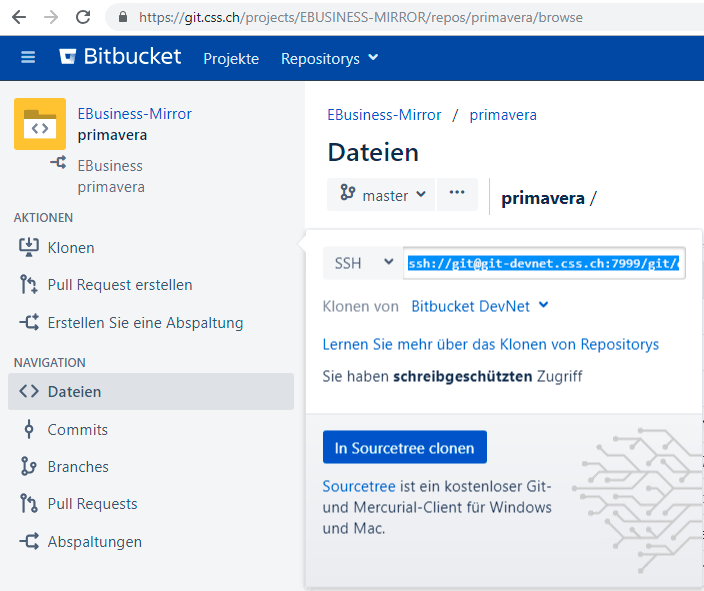
\includegraphics[scale=0.3]{assets/clone.png}

Für das Projekt \code{primavera} ergibt sich dann die git-url \\
\code{ssh://git@git-devnet.css.ch:7999/git/ebusiness-mirror/primavera.git}. Das Klonen erfolgt wie gewohnt mit dem Befehl \\
\code{git clone ssh://git@git-devnet.css.ch:7999/git/ebusiness-mirror/primavera.git}

\subsection{SSH-Schlüssel hinterlegen}
Der soeben erzeugte öffentliche SSH-Schlüssel sollte im Bitbucket hinterlegt werden, um den Transport der Daten über das SSH-Protokoll zu ermöglichen.

\href{https://git.css.ch/plugins/servlet/ssh/account/keys}{https://git.css.ch/plugins/servlet/ssh/account/keys}

Dezidierte Informationen finden sich unter ...TODO...

\subsection{Maven konfigurieren}
\href{https://confluence.css.ch/confluence/display/TEA/Maven+Zugriff+auf+Artifactory+aus+dem+DevNet}{Maven Zugriff auf Artifactory aus dem DevNet}
\begin{itemize}
	\item Den Block \code{settings.xml} auf der Confluenceseite kopieren
	\item Eine neue Datei \code{settings.xml} im Verzeichnis \code{~/.m2} anlegen
	\item Den soeben kopierten Konfigurationsblock in die Datei kopieren und die Datei speichern.
	\item An JFrog-Artifactory im DEVNET unter der URL \\
	\url{https://artifactory-devnet.css.ch/artifactory/webapp/#/home}
	anmelden und das verschlüsselte Passwort ermitteln.
	\item Benutzerlogin (p-Nummer) und verschlüsseltes Passwort in der soeben erzeugten Datei settings.xml anpassen.
\end{itemize}

\begin{bashcode}
# sed -i.bak -E 's!(<username>)[^<]*(</username>)!\1<Deine Login ID>\2!g' ~/.m2/settings.xml, z.B.
sed -i.bak -E 's!(<username>)[^<]*(</username>)!\1p123123\2!g' ~/.m2/settings.xml
\end{bashcode}

\subsection{npm konfigurieren}
Aktuell nicht weiter konfigurieren >>>
~\.npmrc
registry=http://artifactory.css.ch/artifactory/api/npm/npm/
sass\textunderscore binary\textunderscore site=http://repo.iasrv.css.ch/tools/node\textunderscore sass\textunderscore bindings
<<<

\printbibliography
\end{document}
